
\section*{Thể tích}
\subsection{Tóm tắt lý thuyết}
\begin{tomtat}
	\begin{dn}
		Phần không gian được giới hạn bởi hình chóp, hình chóp cụt đều, hình lăng trụ, hình hộp tương ứng được gọi là khối chóp, khối chóp cụt đều, khối lăng trụ, khối hộp. Đỉnh, mặt, cạnh, đường cao của các khối đó lần lượt là đỉnh, cạnh, đường cao của hình chóp, hình chóp cụt đều, hình lăng trụ, hình hộp tương ứng.
		\begin{itemize}
			\item Thể tích của khối chóp có diện tích đáy $S$ và chiều cao $h$ là $V=\dfrac{1}{3}\cdot h\cdot S$.
			\item Thể tích của khối chóp cụt đều có diện tích đáy lớn $S$, diện tích đáy bé $S'$ và chiều cao $h$ là $V=\dfrac{1}{3}\cdot h\cdot (S+S'+\sqrt{S\cdot S'})$.
			\item Thể tích của khối lăng trụ có diện tích đáy $S$ và chiều cao $h$ là $V=h\cdot S$.
		\end{itemize}
	\end{dn}
	\begin{minipage}[t]{0.25\textwidth}
		\begin{tikzpicture}[scale=.6,font=\footnotesize,line join = round, line cap = round, >= stealth]
			%\draw[opacity=0.3] (0,0) grid (6,6);
			\def\x{4} \def\y{2} \def\z{3.5}
			\def\g{-120}
			\coordinate (A) at (0,0);
			\coordinate (E) at ($(A)+(0:\x)$);
			\coordinate (B) at ($(A)+(-60:1.3)$);
			\coordinate (C) at ($(B)+(-30:1)$);
			\coordinate (D) at ($(C)+(20:2)$);
			\coordinate (H) at ($(A)+(-30:1.5)$);
			\coordinate (S) at ($(H)+(90:\z)$);
			
			
			\draw (S)--(A)--(B)--(C)--(D)--(E)--(S)--(D)
			(B)--(S)--(C)
			;
			\draw[dashed] (A)--(E) (S)--(H) 
			;
			\foreach \p/\g in {S/100,A/180,B/-90,C/-70,D/-20,E/0,H/-90} \draw[fill] (\p) circle(.5pt)
			node [shift={(\g:.3)}] {$\p$}
			;
			\draw (1.15,1)node{$h$}
			;
			\draw (1.3,-3)node{$V=\dfrac{1}{3}\cdot h\cdot S$};
		\end{tikzpicture}
	\end{minipage}
	\begin{minipage}[t]{0.25\textwidth}
		\begin{tikzpicture}[scale=.6,font=\footnotesize,line join = round, line cap = round, >= stealth]
			%\draw[opacity=0.3] (0,0) grid (6,6);
			\def\x{4} \def\y{2} \def\z{3.5}
			\def\g{-120}
			\coordinate (A) at (0,0);
			\coordinate (B) at ($(A)+(0:\x)$);
			\coordinate (D) at ($(A)+(40:\y)$);
			\coordinate (C) at ($(B)+(D)-(A)$);
			\coordinate (H) at ($(A)!1/2!(C)$);
			\coordinate (S) at ($(H)+(90:\z)$);
			
			\coordinate (A') at ($(S)!0.4!(A)$);
			\coordinate (B') at ($(S)!0.4!(B)$);
			\coordinate (C') at ($(S)!0.4!(C)$);
			\coordinate (D') at ($(S)!0.4!(D)$);
			\coordinate (H') at ($(S)!0.4!(H)$);
			\draw (2.5,2)node{$h$}
			;
			\draw (A')--(B')--(C')--(D')--
			(A')--(A)--(B)--(C)--(C')
			(B)--(B') (A')--(C') (B')--(D')
			;
			\draw[dashed] (A)--(D)--(C)--(A) (B)--(D)--(D')
			(H)--(H')
			;
			\foreach \p/\g in {A/-100,B/-90,C/0,D/180,H/-90,A'/180,B'/-30,C'/0,D'/180,H'/90} \draw[fill] (\p) circle(.5pt)
			node [shift={(\g:.3)}] {$\p$}
			;
			\draw (2.5,-2)node{$V=\dfrac{1}{3}\cdot h\cdot (S+S'+\sqrt{S\cdot S'})$};
		\end{tikzpicture}
	\end{minipage}
	\begin{minipage}[t]{0.25\textwidth}
		\begin{tikzpicture}[scale=0.7,font=\footnotesize,line join = round, line cap = round, >= stealth]
			%\draw[opacity=0.3] (0,0) grid (6,6);
			\def\x{4} \def\y{2} \def\z{3.5}
			\def\g{-120}
			\coordinate (A) at (0,0);
			\coordinate (B) at ($(A)+(0:\x)$);
			\coordinate (C) at ($(A)+(40:\y)$);
			\coordinate (H) at ($(A)+(10:2.3)$);
			\coordinate (B') at ($(H)+(90:\z)$);
			\coordinate (A') at ($(A)+(B')-(B)$);
			\coordinate (C') at ($(A')+(C)-(A)$);
			
			\draw (A')--(B')--(C')--cycle
			(A')--(A)--(B)--(B')
			;
			\draw[dashed] (C')--(C)--(A) (C)--(B) (B')--(H)
			;
			\foreach \p/\g in {A/-100,B/-80,C/30,H/180,A'/180,B'/80,C'/90} \draw[fill] (\p) circle(.5pt)
			node [shift={(\g:.3)}] {$\p$};
			\draw (2,2)node{$h$}
			;
			\draw (2,-2)node{$V=h\cdot S$};
		\end{tikzpicture}
	\end{minipage}
	\\
	\textbf{Nhận xét}
	\begin{itemize}
		\item Thể tích khối tứ diện bằng một phần ba tích của chiều cao từ một đỉnh và diện tích mặt đối diện với đỉnh đó.
		\item Thể tích của khối hộp bằng tích của một mặt và chiều cao của khối hộp ứng với mặt đó.
	\end{itemize}
	
\end{tomtat}
\subsection{Các dạng toán thường gặp}
\begin{dang}{Thể tích khối chóp, lăng trụ}
	\begin{itemize}
		\item Thể tích của khối chóp có diện tích đáy $S$ và chiều cao $h$ là $V=\dfrac{1}{3}\cdot h\cdot S$.
		\item Thể tích của khối lăng trụ có diện tích đáy $S$ và chiều cao $h$ là $V=h\cdot S$.
	\end{itemize}
\end{dang}
\Opensolutionfile{ans}[ans/ans-1K7-27-Dang1-2]
\subsubsection{Ví dụ mẫu}
\begin{vd}%[1K7YQ-1]
	Cho hình chóp tam giác $S.ABC$ có $SA$, $AB$, $AC$ đôi một vuông góc nhau. Biết độ dài ba cạnh $SA$; $AB$; $AC$ lần lượt là $3$; $4$; $5$. Tính thể tích $V$ của khối chóp $S.ABC$.
	\choice
	{$V=30$}
	{$V=20$}
	{$V=60$}
	{\True $V=10$}
	\loigiai{
		\immini{Diện tích tam giác $ABC$ là $S_{ABC}=\dfrac{1}{2}\cdot AB\cdot AC=\dfrac{1}{2}\cdot 4\cdot 5=10$.\\
			Thể tích khối chóp là $V=\dfrac{1}{3}\cdot S_{ABC}\cdot SA=\dfrac{1}{3}\cdot 10\cdot 3=10$.}{\begin{tikzpicture}[scale=1, font=\footnotesize, line join=round, line cap=round,>=stealth]
				\path (0,0)coordinate (A) (3,0) coordinate (C) (0.7,-0.7) coordinate (B) ($(A)+(0,2)$) coordinate (S);
				\draw (S)--(A)--(B)--(C)--cycle (S)--(B);
				\draw[dashed] (A)--(C);
				\foreach \p/\g in {A/180,B/-90,C/0,S/90} \fill[black] (\p) circle(1pt)+(\g:0.3) node{$\p$};
				\draw pic[draw, angle radius=0.2cm]{right angle=S--A--B} pic[draw, angle radius=0.2cm]{right angle=S--A--C} pic[draw, angle radius=0.2cm]{right angle=C--A--B};
		\end{tikzpicture}}
	}
\end{vd}


\begin{vd}%[1K7YQ-1]
	Cho khối chóp $S.ABC$ có đáy $ABC$ là tam giác đều cạnh $a$, $SA$ vuông góc với mặt phẳng đáy và $SA=2a$. Tính thể tích khối chóp $S.ABC$.
	\choice	
	{$\dfrac{a^3\sqrt{3}}{4}$}
	{\True $\dfrac{a^3\sqrt{3}}{6}$}
	{$\dfrac{a^3\sqrt{3}}{12}$}	
	{$\dfrac{a^3\sqrt{3}}{3}$}
	\loigiai{
		\immini{
			Thể tích của khối chóp là $V=\dfrac{1}{3}S_{ABC}\cdot SA=\dfrac{1}{3}\cdot\dfrac{a^2\sqrt{3}}{4}\cdot 2a=\dfrac{a^3\sqrt{3}}{6}$.
		}{
			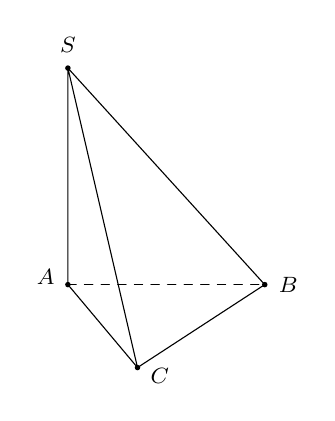
\begin{tikzpicture}[line join=round,line cap=round, font=\footnotesize,scale=1,>=stealth]
				\def\r{2.5}
				\path
				(0,0) coordinate (A)
				(\r,0) coordinate (B)		
				(-50:0.55*\r) coordinate (C)
				(90:1.1*\r) coordinate (S)					
				;
				\draw (S)--(B)-- (C) --(A)--(S)--(C);
				\draw[dashed] (A)--(B);
				\foreach \x/\g in {A/160,B/0,C/-20,S/90}\fill[black] (\x) circle(1pt)+(\g:0.3)node{$\x$};	
			\end{tikzpicture}
		}
	}
\end{vd}
\begin{vd}%[1K7YQ-1]
	Cho khối chóp $S.ABCD$ có đáy $ABCD$ là hình vuông cạnh bằng $a$, cạnh bên $SA$ vuông góc với mặt đáy và $SA=3a$. Thể tích của khối chóp $S$. $ABCD$ bằng
	\choice
	{$\dfrac{1}{3}a^3$}
	{$3a^3$}
	{\True $a^3$}
	{$9a^3$}
	\loigiai{
		\immini{
			Khối chóp đã cho có
			$$\begin{aligned}
				&\bullet~\text{chiều cao } h=SA=3a\\
				&\bullet~ \text{diện tích mặt đáy } S_{ABCD}=a^2.
			\end{aligned}$$
			Vậy $V_{S.ABCD}=\dfrac{1}{3} \cdot 3a \cdot a^2=a^3$.}
		{\vspace{-0.5cm}
			\begin{tikzpicture}[scale=0.6, font=\footnotesize, line join=round, line cap=round]
				\foreach \x\y\t in {0/3/S,0/0/A,-1.3/-1.6/B,2.5/-1.6/C}
				\coordinate (\t) at (\x,\y);
				\coordinate (D) at ($(A)+(C)-(B)$);
				\draw (S)--(C)--(B)--(S)--(D)--(C);
				\draw[dashed](S)--(A) (B)--(A)--(D);
				\path pic[draw,angle radius=4]{right angle=S--A--B}
				pic[draw,angle radius=6]{right angle=S--A--D};
				\foreach \t/\g in {S/90,A/160,B/-130,C/-60,D/0}
				\draw[fill=black] (\t) circle(1pt)
				node[shift={(\g:7pt)}]{$\t$};
		\end{tikzpicture}}
	}
\end{vd}
\begin{vd}%[1K7BQ-1]
	Cho khối chóp $S.ABCD$ có đáy $ABCD$ là hình vuông cạnh $a$, $SA\perp(ABCD)$. Tính thể tích của khối chóp biết góc giữa $SC$ và $(ABCD)$ bằng $45^{\circ}$. 
	\choice
	{$\dfrac{a^3\sqrt{2}}{6}$}
	{$\dfrac{a^3\sqrt{2}}{4}$}
	{$a^3\sqrt{2}$}
	{\True $\dfrac{a^3\sqrt{2}}{3}$}
	\loigiai{
		\immini{
			Vì $SA\perp(ABCD)$ nên $AC$ là hình chiếu của $SC$ trên $(ABCD)$.\\
			Do đó $45^{\circ}=\left(SC,(ABCD)\right)=(SC,AC)=\widehat{SCA}$.\\
			$\Rightarrow$ Tam giác $SAC$ vuông cân đỉnh $A\Rightarrow SA=AC=a\sqrt{2}$.\\
			Vậy $V_{S.ABCD}=\dfrac{1}{3}SA\cdot S_{ABCD}=\dfrac{1}{3}\cdot a\sqrt{2}\cdot a^2=\dfrac{a^3\sqrt{2}}{3}$.
		}{
			\begin{tikzpicture}[scale=0.7, font=\footnotesize, line join=round, line cap=round,>=stealth]
				\path
				(0,0) coordinate (A)
				(-1.3,-1.6) coordinate (B)
				(2.5,-1.6)coordinate (C)
				($(A)+(C)-(B)$) coordinate (D)
				($(A)+(0,3)$) coordinate (S)
				;
				\draw (S)--(B)--(C)--(D)--cycle (S)--(C);
				\draw[dashed] (S)--(A)--(D) (C)--(A)--(B);	
				\foreach \p/\q in {S/90,A/-90,B/-90,C/-90,D/0}			
				\fill[black] (\p) circle (1.0pt)node[shift={(\q:2.5mm)}]{$\p$};
			\end{tikzpicture}
		}
	}
\end{vd}
\begin{vd}%[1K7BQ-1]
	Cho hình chóp $S . A B C$ có đáy $A B C$ là tam giác vuông tại $A$ và có $A B=a, B C=a \sqrt{3}$. Mặt bên $S A B$ là tam giác đều và nằm trong mặt phẳng vuông góc với mặt phẳng $(A B C)$. Tính theo $a$ thể tích của khối chóp $S . A B C$.
	\choice
	{$V=\dfrac{a^3 \sqrt{6}}{4}$}
	{$V=\dfrac{a^3 \sqrt{6}}{8}$}
	{\True$V=\dfrac{a^3 \sqrt{6}}{12}$}
	{$V=\dfrac{a^3 \sqrt{6}}{6}$}
	\loigiai{
		\begin{center}
			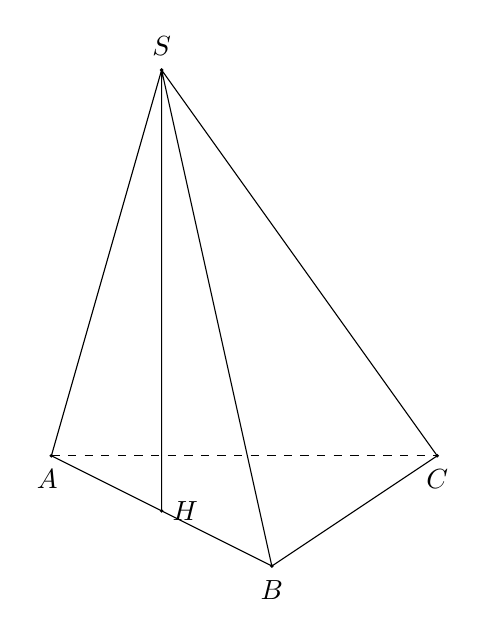
\begin{tikzpicture}[scale=0.7]%Hình
				\path
				(0,0) coordinate (A)
				(4,-2) coordinate (B)
				(7,0) coordinate (C)
				(2,-1) coordinate (H)
				(2,7) coordinate (S);
				\draw (0,0)--(4,-2)--(7,0) (2,7)--(0,0) (2,7)--(4,-2) (2,7)--(7,0) (2,7)--(2,-1);
				\draw[dashed] (0,0)--(7,0);
				\foreach \p/\q in {S/90,A/-100,B/-90,C/-90,H/0}
				\fill[black] (\p) circle (1.0pt)node[shift={(\q:3mm)}]{$\p$};
				%				\tkzMarkRightAngle(B,A,C)
				%				\tkzMarkRightAngle(S,H,A)
			\end{tikzpicture}	
		\end{center}
		Ta có: $AC^2=BC^2-AB^2=3a^2-a^2=2a^2\Rightarrow AC=a\sqrt{2}$.\\
		$SH$ là đường cao của tam giác đều cạnh $a$ nên $SH=\dfrac{a\sqrt{3}}{2}$.\\
		Diện tích tam giác $ABC$: $S=\dfrac{1}{2}\cdot AB\cdot AC=\dfrac{1}{2}\cdot a\cdot a\sqrt{2}=\dfrac{a^2\sqrt{2}}{2}$.\\
		Thể tích của khối chóp $S. ABC$ là $V=\dfrac{1}{3}\cdot SH\cdot S_{ABC}=\dfrac{1}{3}\cdot \dfrac{a\sqrt{3}}{2}\cdot \dfrac{a^2\sqrt{2}}{2}=\dfrac{a^3\sqrt{6}}{12}$.\\
	}
\end{vd}

\begin{vd}%[1K7KQ-1]
	Cho hình chóp $S.ABCD$ có đáy là hình vuông cạnh $a$, mặt bên $SAB$ cân tại $S$ nằm trong mặt phẳng vuông góc với $(ABCD)$, góc giữa cạnh bên $\mathrm{SB}$ và mặt đáy là $60^{\circ}$. Tính thể tích $V$ của khối chóp $S.ABCD$.
	\choice
	{\True $V=\dfrac{\sqrt{3}a^3}{6}$}
	{$V=\dfrac{2 \sqrt{3}a^3}{6}$}
	{$V=\dfrac{a^3}{3}$}
	{$V=\dfrac{2 \sqrt{3}a^3}{9}$}
	\loigiai{
		\immini{
			Hai mặt phẳng $(SAB)$, $(ABCD)$ vuông góc và cắt nhau theo giao tuyến $AB$ nên gọi $H$ là hình chiếu của $S$ trên $AB$ thì $H$ là hình chiếu của $S$ trên $(ABCD)$.\\ Mặt khác, tam giác $(SAB)$ cân tại $S$ nên $H$ là trung điểm của $AB$.\\
			$BH$ là hình chiếu của là hình chiếu của $SB$ trên $(ABCD)$ nên góc giữa $SB$ và $(ABCD)$ là góc giữa hai đường thẳng $SB$, $BH$. \\
			Tam giác $SBH$ vuông tại $H$, $BH=\dfrac{a}{2}$, $\widehat{SBH}=(SB,BH)=60^\circ$.\\
			Suy ra $SH=BH\cdot \tan \widehat{SBH}=\dfrac{a}{2}\cdot \tan 60^\circ=\dfrac{a\sqrt{3}}{2}$.\\
			Vậy thể tích của khối chóp $S.ABCD$ là $$V=\dfrac{1}{3}\cdot S_{ABCD}\cdot SA=\dfrac{1}{3}\cdot a^2 \cdot \dfrac{a\sqrt{3}}{2} =\dfrac{a^3\sqrt{3}}{6}.$$ }{\begin{tikzpicture}[line cap=round,line join=round, >=stealth,scale=1]
				\def \a{-2} \def \b{-1} \def \c{4} \def \h{4} 
				\path (.5,.5)coordinate(A) 
				+(\a,\b)coordinate(B)
				+(\c,0)coordinate(D)
				($(B)+(D)-(A)$)coordinate(C)
				($(A)!1/2!(B)$)coordinate(H)
				+(0,\h)coordinate(S);
				%\draw[ultra thin,color=gray] (-2.5,-1.5) grid (5.5,4.5);
				\draw [dashed] (B)--(A)--(D) (A)--(S) (S)--(H)--(C);
				\draw [thick](S)--(B)--(C)--(D)--(S)--(C);
				\foreach \d/\g in {S/90,A/60,B/160,C/-90,D/0,H/60}
				\fill[black](\d) circle (1pt)+(\g:.38)node{$\d$};
				\foreach \x/\o/\y/\r in {S/H/B/2,S/H/C/2,A/B/C/2} \draw ($(\o)!\r mm!(\x)$)--($($(\o)!\r mm!(\x)$)+($(\o)!\r mm!(\y)$)-(\o)$)--($(\o)!\r mm!(\y)$);
				\draw[-] ($(B)!4mm!(A)$) to[bend right=45]  ($(B)!4mm!(S)$) ($(B)+(45:0.7)$)node{$60^\circ$};
	\end{tikzpicture}}}
\end{vd}
\begin{vd}%[1K7BQ-1]
	Cho khối chóp tam giác đều $S.ABC$ có cạnh đáy $AB=2a$, cạnh bên $SA=a\sqrt{2}$. Thể tích khối chóp đã cho bằng
	\choice
	{$\sqrt{2}a^3$}
	{\True $\dfrac{\sqrt{2}}{3}a^3$}
	{$\dfrac{\sqrt{2}}{6}a^3$}
	{$\dfrac{\sqrt{2}}{2}a^3$}
	\loigiai{
		\immini{Gọi $H$ là trọng tâm của tam giác $ABC$ và $M$ là trung điểm $BC$.\\
			Ta có $AM=a\sqrt{3} \Rightarrow AH=\dfrac{2}{3}AM=\dfrac{2\sqrt{3}}{3}a$.\\
			Mặt khác $SH=\sqrt{SA^2-AH^2}=\sqrt{\left(\sqrt{2}a\right)^2-\left(\dfrac{2\sqrt{3}a}{3}\right)^2}=\dfrac{\sqrt{6}}{3}a$.\\
			Vậy thể tích khối chóp đã cho là $$V=\dfrac{1}{3}S_{ABC}\cdot SH=\dfrac{1}{3}\cdot(2a)^2\cdot \dfrac{\sqrt{3}}{4}\cdot \dfrac{\sqrt{6}a}{3}=\dfrac{\sqrt{2}a^3}{3}.$$}
		{\begin{tikzpicture}[scale=1, font=\footnotesize,>=stealth]
				%Gán số liệu.
				\def\canhAC{4};\def\canhBA{2};\def\gocBAC{-50};\def\h{3.5};
				%Gán tọa độ.
				\coordinate (A) at (0,0);
				\coordinate (B) at ($(A)+(\gocBAC:\canhBA)$);
				\coordinate (C) at ($(A)+(0:\canhAC)$);
				\coordinate (O) at ($ 1/3*(A)+1/3*(B)+1/3*(C) $);
				\coordinate (S) at ($(O)+(90:\h)$);
				\coordinate (M) at ($(B)!0.5!(C)$);
				\coordinate (N) at ($(A)!0.5!(B)$);
				\coordinate (H) at (intersection of A--M and C--N);
				%Vẽ khối chóp S.ABC đều.
				\draw (S)--(B) (S)--(A)--(B) (S)--(C)--(B);
				\draw[dashed] (A)--(C) (A)--(M) (C)--(N) (S)--(H);
				%Gán nhãn.
				\foreach \x/\y in {S/90,A/180,B/-90,C/0,M/-10,N/190,H/-60}{\fill (\x) circle (1pt) ($(\x)+(\y:0.3cm)$) node{$\x$};}
				%Kí hiệu
				\path (A)--(N)node[sloped, midway]{\tiny |};
				\path (N)--(B)node[sloped, midway]{\tiny |};
				\path (C)--(M)node[sloped, midway]{\tiny ||};
				\path (M)--(B)node[sloped, midway]{\tiny ||};
		\end{tikzpicture}}
	}
\end{vd}

\begin{vd}%[1K7BQ-1]
	Thể tích của khối chóp tứ giác đều có tất cả các cạnh bằng $a$ là
	\choice
	{$\dfrac{a^3\sqrt{2}}{4}$}
	{\True $\dfrac{a^3\sqrt{2}}{6}$}
	{$\dfrac{a^3\sqrt{2}}{3}$}
	{$\dfrac{a^3\sqrt{2}}{2}$}
	\loigiai{
		\immini{
			Xét hình chóp $S.ABCD$ đều cạnh $a$, có tâm ở đáy là $O\Rightarrow SO\perp (ABCD)$.\\
			Ta có $SA^2+SC^2=2a^2=AC^2$ nên tam giác $SAC$ vuông tại $S$, do đó $SO=\dfrac{AC}{2}=\dfrac{a\sqrt{2}}{2}$.\\
			Vậy $V_{S.ABCD}=\dfrac{1}{3}\cdot SO\cdot S_{ABCD}=\dfrac{1}{3}\cdot \dfrac{a\sqrt{2}}{2}\cdot a^2=\dfrac{a^3\sqrt{2}}{6}$. 
		}{
			\begin{tikzpicture}[scale=1, font=\footnotesize, line join=round, line cap=round,>=stealth]
				\path
				(0,0) coordinate (A)
				(-1.9,-1.6)coordinate (B)
				(1.6,-1.6)coordinate (C)
				($(A)+(C)-(B)$)coordinate (D)
				($(A)!0.5!(C)$)coordinate (O)
				($(O)+(0,3.5)$) coordinate (S)
				;
				\draw (S)--(B)--(C)--(D)--cycle (S)--(C);
				\draw[dashed] (O)--(S)--(A)--(D) (C)--(A)--(B)--(D);	
				\foreach \p/\q in {S/90,A/-100,B/-90,C/-90,D/0,O/-90}
				\fill[black] (\p) circle (1.0pt)node[shift={(\q:3mm)}]{$\p$};
				\draw pic[draw=black,angle radius=0.2cm] {right angle = S--O--A}; 
				\draw pic[draw=black,angle radius=0.2cm] {right angle = S--O--D}; 		
			\end{tikzpicture}
		}
	}
\end{vd}
\begin{vd}%[1K7BQ-1]
	Cho hình chóp đều $S . A B C D$ có cạnh bên $S A=4$ và tạo với đáy một góc bằng $45^{\circ}$. Thể tích của khối chóp đó bằng
	\choice
	{$\dfrac{16 \sqrt{2}}{3}$}
	{$32 \sqrt{3}$}
	{$16 \sqrt{3}$}
	{\True $\dfrac{32 \sqrt{2}}{3}$}
	\loigiai{\begin{center}
			\begin{tikzpicture}[scale=1, font=\footnotesize, line join=round, line cap=round, >=stealth]
				\def\bc{4} % cạnh BC
				\def\ba{2} % cạnh BA
				\def\h{4} % đường cao
				\def\gocB{30} % góc B của đáy
				\coordinate[label=below left:$B$] (B) at (0,0);
				\coordinate[label=above right:$A$] (A) at (\gocB:\ba);
				\coordinate[label=below:$C$] (C) at (\bc,0);
				\coordinate[label=right:$D$] (D) at ($(C)-(B)+(A)$);
				\coordinate[label=below:$O$] (O) at ($(A)!.5!(C)$);
				\coordinate[label=above:$S$] (S) at ($(O)+(90:\h)$);
				\draw (B)--(C)--(D)--(S)--cycle (S)--(C);
				\draw[dashed] (C)--(A)--(D)--(B) (O)--(S)--(A)--(B);
				\foreach \diem in {A,B,C,D,S,O}	\fill (\diem)circle(1.5pt);
			\end{tikzpicture}
			
		\end{center}
		Theo giả thiết, $\widehat{SAO}=45^\circ$ nên tam giác $SAC$ vuông cân tại $S$ suy ra $AC=4\sqrt{2}$ và $SO=2\sqrt{2}$.\\
		Khi đó $AB=4$.\\
		Thể tích của khối chóp là $V=\dfrac{1}{3}\cdot4^2\cdot2\sqrt{2}=\dfrac{32\sqrt{2}}{3}$.
	}
\end{vd}
\begin{vd}%[1K7YQ-1]
	Cho khối lăng trụ đứng $A B C \cdot A' B' C'$ có đáy là tam giác đều cạnh $a$ và $A A'=2 a$. Thể tích của khối lăng trụ đã cho bằng
	\choice
	{$\dfrac{\sqrt{3} a^{3}}{3}$}
	{\True $\dfrac{\sqrt{3} a^{3}}{2}$}
	{$\dfrac{\sqrt{3} a^{3}}{6}$}
	{$\sqrt{3} a^{3}$}
	\loigiai{
		\immini{
			Khối lăng trụ đứng có $h=AA'=2a$ và diện tích đáy $S_{ABC}=\dfrac{a^2\sqrt{3}}{4}$.\\
			Vậy thể tích của khối lăng trụ $V=S_{ABC}\cdot h=\dfrac{a^2\sqrt{3}}{4}\cdot 2a=\dfrac{\sqrt{3} a^{3}}{2}$.
		}{
			\begin{tikzpicture}[scale=0.7, font=\footnotesize, line join=round, line cap=round, >=stealth]
				\def\h{1.5}
				\path
				(0,0) coordinate (A)
				(2,-1) coordinate (B)
				(3,0) coordinate (C)
				($(A)+(0,\h)$) coordinate (A')
				($(A')+(B)$) coordinate (B')
				($(A')+(C)$) coordinate (C')
				;
				\draw (B)--(B')--(A')--(A)--(B)--(C)--(C')--(B') (A')--(C');
				\draw[dashed] (A)--(C);
				\foreach \d/\g in {A/-170,B/-90,C/-20,A'/170,B'/90,C'/20}{
					\draw[fill=black](\d) circle (1pt) +(\g:.3)node{$\d$};}
				
		\end{tikzpicture}}
	}
\end{vd}
\begin{vd}%[1K7YQ-1]
	Cho hình lăng trụ tứ giác đều $ABCD.A'B'C'D'$ có $AB=3$, $AB'=5$. Tính thể tích $V$ của khối lăng trụ $ABCD.A'B'C'D'$.
	\choice
	{$V=45$}
	{$V=18$}
	{$V=48$}
	{\True $V=36$}
	\loigiai{
		\immini{Vì $ABCD.A'B'C'D'$ là lăng trụ tứ giác đều nên $B'B\perp (ABCD)$.\\
			Ta tính được $B'B=\sqrt{AB'^2-AB^2}=4$.\\
			Thể tích khối lăng trụ $ABCD.A'B'C'D'$ là $V=AB^2\cdot B'B=3^2\cdot 4=36$.}{\begin{tikzpicture}[scale=1, font=\footnotesize, line join=round, line cap=round,>=stealth]
				\path (0,2.5) coordinate (h) (0,0)coordinate (B) (2.3,0) coordinate (C) (3.5,0.7) coordinate (D) ($(B)+(D)-(C)$) coordinate (A);
				\foreach \p in {A,B,C,D}\path ($(\p)+(h)$) coordinate (\p');
				\draw (A')--(B')--(B)--(C)--(D)--(D')--cycle (B')--(C')--(D') (C)--(C');
				\draw[dashed] (B)--(A)--(D) (B')--(A)--(A');
				\foreach \p/\g in {A/45,B/240,C/-60,D/0,A'/90,B'/180,C'/-30,D'/45} \fill[black] (\p) circle(1pt)+(\g:0.3) node{$\p$};
				\draw pic[draw, angle radius=0.2cm]{right angle=B'--B--A};
		\end{tikzpicture}}
	}
\end{vd}


\begin{vd}%[1K7KQ-1]
	Cho hình lăng trụ tam giác đều $ABC.A'B'C'$ có cạnh đáy $AB=a$, góc giữa hai mặt phẳng $(A'BC)$ và $(ABC)$ là $45^{\circ}$. Khi đó thể tích khối lăng trụ $ABC.A'B'C'$ là
	\choice
	{$\dfrac{2a^3}{3}$}
	{$\dfrac{a^3}{3}$}
	{\True $\dfrac{3a^3}{8}$}
	{$a^3$}
	\loigiai{
		\immini{Vì $ABC.A'B'C'$ là lăng trụ tam giác đều nên $A'A\perp (ABC)$.\\
			Gọi $M$ là trung điểm của $BC$, ta có $AM\perp BC$.\\
			Tiếp đến $(A'BC)\cap (ABC)=BC$ nên góc giữa mặt phẳng $(A'BC)$ với $(ABC)$ là $\widehat{A'MA}=45^\circ$.\\
			Ta tính được $AM=\dfrac{a\sqrt{3}}{2}$, $A'A=AM=\dfrac{a\sqrt{3}}{2}$.\\
			Diện tích tam giác $ABC$ là $S_{ABC}=\dfrac{a^2\sqrt{3}}{4}$.\\
			Vậy thể tích của khối lăng trụ $ABC.A'B'C'$ là $V=S_{ABC}\cdot A'A=\dfrac{3a^3}{8}$.}{\begin{tikzpicture}[scale=1, font=\footnotesize, line join=round, line cap=round,>=stealth]
				\path (0,0)coordinate (A) (3,0) coordinate (C) (1.3,-1) coordinate (B) (0,3) coordinate (h) ($(B)!0.5!(C)$) coordinate (M);
				\foreach \p in {A,B,C} {\draw (\p)--(\p)--+(h) coordinate (\p');}
				\draw (A')--(B')--(C')--cycle (A)--(B)--(C) (A')--(B);
				\draw[dashed] (A)--(C)--(A')--(M)--(A);
				\foreach \p/\g in {A/180,B/-90,C/0,A'/180,B'/-30,C'/0,M/-45} \fill[black] (\p) circle(1pt)+(\g:0.3) node{$\p$};
				\draw pic[draw, angle radius=0.2cm]{right angle=A--M--B} pic[draw, angle radius=0.2cm]{right angle=A'--A--M};
				\draw pic[draw, "$45^\circ$", angle eccentricity=1.4, angle radius=0.4cm]{angle=A'--M--A};
		\end{tikzpicture}}
	}
\end{vd}
\begin{vd}%[1K7KQ-1]
	Một khối lăng trụ tam giác có đáy là tam giác đều cạnh $3$ cm, cạnh bên bằng $2 \sqrt{3}$ cm tạo với mặt phẳng đáy một góc $30^{\circ}$. Khi đó thể tích $V$ của khối lăng trụ là
	\choice
	{$V=\dfrac{9}{4}\mathrm{cm}^3$}
	{$V=\dfrac{27 \sqrt{3}}{4}\mathrm{cm}^3$}
	{$V=\dfrac{9 \sqrt{3}}{4}\mathrm{cm}^3$}
	{\True $V=\dfrac{27}{4}\mathrm{cm}^3$}
	\loigiai{
		\immini
		{
			Gọi $ABC.A'B'C'$ là khối lăng trụ đang xét, $H$ là hình chiếu của $A'$ lên $(ABC)$.\\
			Từ giả thiết ta có $\widehat{A'AH}=30^{\circ}$.\\
			Ta có $\sin 30^{\circ}=\dfrac{A'H}{AA'}\Rightarrow A'H=A A'\cdot \sin 30^{\circ}=\sqrt{3}$ cm.\\
			Thể tích khối lăng trụ là\\
			$V=A A'\cdot S_{A B C}=\sqrt{3}\cdot \dfrac{3^2 \sqrt{3}}{4}=\dfrac{27}{4}$ cm$^3$.
		}
		{
			\begin{tikzpicture}[scale=1, font=\footnotesize, line join=round, line cap=round, >=stealth]
				\def\ac{4} % cạnh AC
				\def\ab{2} % cạnh AB
				\def\h{4} % chiều cao
				\def\gocA{50} % góc A của đáy
				\path
				(0,0) coordinate (A)
				(\ac,0) coordinate (C)
				(-\gocA:\ab) coordinate (B)
				($(A)+(80:\h)$) coordinate (A')
				($(B)-(A)+(A')$) coordinate (B')
				($(C)-(A)+(A')$) coordinate (C')
				($(A)+(20:1)$) coordinate (H);
				\draw
				pic[draw,angle radius=7]{right angle=A--H--A'}
				(A')--(A)--(B)--(C)--(C')--(A')--(B')--(C') (B)--(B');
				\draw[dashed] (A)--(C) (A)--(H)--(A');
				\foreach \x/\g in {A/180,B/-90,C/0,A'/180,C'/0,B'/-40,H/-30}\fill (\x) circle (1pt)+(\g:3mm) node{$ \x $};
			\end{tikzpicture}
		}
	}
\end{vd}
\begin{vd}%[1K7KQ-1]
	Cho hình lăng trụ $ABC.A'B'C'$ có đáy $ABC$ là tam giác đều cạnh là $a$. Tam giác $A'AB$ cân tại $A'$ và nằm trong mặt phẳng vuông góc với mặt đáy, mặt bên $(AA'C'C)$ tạo với mặt phẳng $(ABC)$ một góc $45^{\circ}$. Thể tích của khối lăng trụ $ABC.A'B'C'$ là
	\choice
	{$V=\dfrac{3a^3}{4}$}
	{$V=\dfrac{3a^3}{32}$}
	{\True $V=\dfrac{3a^3}{16}$}
	{$V=\dfrac{3a^3}{8}$}
	\loigiai{
		\immini{
			Gọi $M$, $H$, $K$ lần lượt là trung điểm của $AC$, $AB$, $AM$.\\
			Suy ra $A'H\perp AB$ mà $\heva{&(A'AB)\perp (ABC)\\& (A'AB)\cap (ABC)=AB \\ & A'H\subset (A'AB)}\Rightarrow A'H\perp (ABC)$.\\
			Ta có $\triangle ABC$ đều nên $BM\perp AC\Rightarrow HK\perp AC$.\\
			Do đó $\heva{& A'H\perp AC \\ & HK\perp AC}\Rightarrow A'K\perp AC$.\\
			Mặt khác $\heva{& (AA'C'C) \cap (ABC)=AC \\ & A'K\subset(AA'C'C),A'K\perp AC\\ & HK\subset(ABC),HK\perp AC}$\\
			$\Rightarrow 45^{\circ}=\left((ACC'A'),(ABC)\right)=(A'K,HK)=\widehat{A'KH}$.			
		}{
			\begin{tikzpicture}[scale=1, font=\footnotesize, line join=round, line cap=round,>=stealth]
				\path
				(0,0)coordinate (A)
				(1.6,-2)coordinate (B)
				(4,0)coordinate (C)
				($(A)!0.5!(B)$) coordinate (H)
				($(H)+(0,4)$) coordinate (A')
				($(A')+(B)-(A)$)coordinate (B')
				($(A')+(C)-(A)$)coordinate (C')					
				($(A)!0.5!(C)$) coordinate (M)	
				($(A)!0.5!(M)$) coordinate (K)	
				;
				\draw (A)--(B)--(C)--(C')--(B')--(A')--cycle (H)--(A')--(C') (A')--(B)--(B');
				\draw[dashed] (A)--(C) (B)--(M) (H)--(K)--(A');	
				\foreach \p/\q in {A/180,B/-90,C/0,A'/180,B'/75,C'/0,H/-110,M/80,K/-60}
				\fill[black] (\p) circle (1.0pt)node[shift={(\q:3mm)}]{$\p$};
			\end{tikzpicture}
		}\noindent
		Tam giác $A'HK$ vuông và $\widehat{A'KH}=45^\circ$ nên vuông cân đỉnh $H$, do đó  $A'H=HK=\dfrac{BM}{2}=\dfrac{1}{2}\cdot\dfrac{a\sqrt{3}}{2}=\dfrac{a\sqrt{3}}{4}$.\\
		Vậy $V_{ABC.A'B'C'}=A'H\cdot S_{ABC}=\dfrac{a\sqrt{3}}{4}\cdot \dfrac{a^2\sqrt{3}}{4}=\dfrac{3a^3}{16}$. 
	}
\end{vd}

\subsubsection{Bài tập rèn luyện}
\begin{ex}%[1K7YQ-1]
	Cho khối chóp $S.ABC$ có $SA$ vuông góc với mặt phẳng $(ABC)$. Biết $SA=2a$ và tam giác $ABC$ vuông tại $A$ có $AB=3a$, $AC=4a$. Tính thể tích $V$ của khối chóp $S.ABC$ theo $a$.
	\choice
	{$6a^3$}
	{$8a^3$}
	{\True $4a^3$}
	{$12a^3$}
	\loigiai{
		\immini{Diện tích tam giác $ABC$ là $S_{ABC}=\dfrac{1}{2}\cdot AB\cdot AC=6a^2$.\\
			Thể tích khối chóp $S.ABC$ là $V=\dfrac{1}{3}\cdot S_{ABC}\cdot SA=\dfrac{1}{3}\cdot 6a^2\cdot 2a=4a^3$.}{\begin{tikzpicture}[scale=1, font=\footnotesize, line join=round, line cap=round,>=stealth]
				\path (0,0)coordinate (A) (3,0) coordinate (C) (0.7,-0.7) coordinate (B) ($(A)+(0,2)$) coordinate (S);
				\draw (S)--(A)--(B)--(C)--cycle (S)--(B);
				\draw[dashed] (A)--(C);
				\foreach \p/\g in {A/180,B/-90,C/0,S/90} \fill[black] (\p) circle(1pt)+(\g:0.3) node{$\p$};
				\draw pic[draw, angle radius=0.2cm]{right angle=S--A--B} pic[draw, angle radius=0.2cm]{right angle=S--A--C} pic[draw, angle radius=0.2cm]{right angle=C--A--B};
		\end{tikzpicture}}
	}
\end{ex}
\begin{ex}%[1K7YQ-1]
	Tính thể tích $V$ của khối lăng trụ tam giác đều có tất cả các cạnh bằng $a$.
	\choice
	{$V=\dfrac{a^3\sqrt{2}}{3}$}
	{\True $V=\dfrac{a^3\sqrt{3}}{4}$}
	{$V=\dfrac{a^3\sqrt{2}}{4}$}
	{$V=\dfrac{a^3\sqrt{3}}{2}$}
	\loigiai{
		\immini{
			Khối lăng trụ đã cho là lăng trụ đứng có cạnh bên bằng $a$, đáy là tam giác đều cạnh $a$ nên diện tích mặt đáy bằng $\dfrac{a^2\sqrt{3}}{4}$.\\
			Gọi $V$ là thể tích khối lăng trụ tam giác đều đã cho thì  
			$$V=a \cdot \dfrac{a^2\sqrt{3}}{4}=\dfrac{a^3\sqrt{3}}{4}.$$}
		{\vspace{-0.5cm}
			\begin{tikzpicture}[scale=0.6, font=\footnotesize, line join=round, line cap=round]
				\def\h{3.5}
				\foreach \x\y\t in {0/0/A,1.5/-1/B,3.5/0/C}
				\coordinate (\t) at (\x,\y);
				\coordinate (A') at ($(A)+(0,\h)$);
				\coordinate (B') at ($(B)+(0,\h)$);
				\coordinate (C') at ($(C)+(0,\h)$);
				\draw (B)--(A)--(A')--(C')--(C)--(B)--(B')--(C') (A')--(B');
				\draw[dashed](A)--(C);
				\foreach \t/\g in {A/180,B/-90,C/0,A'/170,B'/80,C'/0}
				\draw[fill=black] (\t) circle(1pt)
				node[shift={(\g:7pt)}]{$\t$};
		\end{tikzpicture}}
	}
\end{ex}
\begin{ex}%[1K7BQ-1]
	\immini
	{
		Cho hình lăng trụ đứng $ABC.A'B'C'$ có đáy $ABC$ là tam giác vuông tại $A$. Biết rằng $AB=3$, $AC=4$, biết $A'C$ tạo với mặt phẳng $(ABC)$ một góc $60^\circ$. Thể tích khối lăng trụ đã cho bằng
		\choice{\True $24\sqrt{3}$}{$8\sqrt{3}$}{$12\sqrt{3}$}{$48\sqrt{3}$}
	}
	{
		\begin{tikzpicture}[scale=0.7, font=\footnotesize, line join=round, line cap=round, >=stealth]
			\def\ac{4} % cạnh AC
			\def\ab{2} % cạnh AB
			\def\h{4} % chiều cao
			\def\gocA{50} % góc A của đáy
			\coordinate[label=left:$A$] (A) at (0,0);
			\coordinate[label=right:$C$] (C) at (\ac,0);
			\coordinate[label=below left:$B$] (B) at (-\gocA:\ab);
			\coordinate[label=left:$A'$] (A') at ($(A)+(90:\h)$);
			\coordinate[label=below left:$B'$] (B') at ($(B)-(A)+(A')$);
			\coordinate[label=right:$C'$] (C') at ($(C)-(A)+(A')$);
			\draw (A')--(A)--(B)--(C)--(C')--(A')--(B')--(C') (B)--(B');
			\draw[dashed] (A)--(C);
			\foreach \diem in {A,B,C,A',B',C'} \fill (\diem)circle(1.5pt);
			
		\end{tikzpicture}
	}
	\loigiai{
		\immini
		{
			Vì $A'A$ vuông góc với $(ABC)$ nên $AC$ là hình chiếu của $A'C$ lên $(ABC)$.\\
			Vậy $(A'C,(ABC))=\widehat{A'CA}$.\\
			Ta có $AA'=AC\tan 60^\circ=4\sqrt{3}$.\\
			Vậy $V_{ABC.A'B'C'}=AA'\cdot S_{ABC}=4\sqrt{3}\cdot \dfrac{1}{2}\cdot 3\cdot 4=24\sqrt{3}$.
		}
		{
			\begin{tikzpicture}[scale=0.7, font=\footnotesize, line join=round, line cap=round, >=stealth]
				\def\ac{4} % cạnh AC
				\def\ab{2} % cạnh AB
				\def\h{4} % chiều cao
				\def\gocA{50} % góc A của đáy
				\coordinate[label=left:$A$] (A) at (0,0);
				\coordinate[label=right:$C$] (C) at (\ac,0);
				\coordinate[label=below left:$B$] (B) at (-\gocA:\ab);
				\coordinate[label=left:$A'$] (A') at ($(A)+(90:\h)$);
				\coordinate[label=below left:$B'$] (B') at ($(B)-(A)+(A')$);
				\coordinate[label=right:$C'$] (C') at ($(C)-(A)+(A')$);
				\draw (A')--(A)--(B)--(C)--(C')--(A')--(B')--(C') (B)--(B');
				\draw[dashed] (A)--(C)--(A');
				\foreach \diem in {A,B,C,A',B',C'} \fill (\diem)circle(1.5pt);
				
			\end{tikzpicture}
		}
	}
\end{ex}
\begin{ex}%[1K7KQ-1]
	Cho khối chóp $S.ABCD$ có đáy là hình thang vuông tại $A$ và $B$. Hai mặt phẳng $(SAB)$ và $(SAD)$ cùng vuông góc với mặt phẳng đáy. Biết $AD=2BC=2a$ và $BD=a\sqrt{5}$. Tính thể tích khối chóp $S.ABCD$ biết góc giữa $SB$ và $(ABCD)$ bằng $30^\circ$.
	\choice
	{$V_{S.ABCD}=\dfrac{4a^3\sqrt{21}}{9}$}
	{\True $V_{S.ABCD}=\dfrac{a^3\sqrt{3}}{6}$}
	{$V_{S.ABCD}=\dfrac{a^3\sqrt{3}}{12}$}
	{$V_{S.ABCD}=\dfrac{a^3\sqrt{3}}{8}$}
	\loigiai{
		\immini
		{
			Từ $\heva{& (SAB)\perp (ABCD) \\ & (SAD)\perp (ABCD)\\& (SAB)\cap (SAD)=SA}\Rightarrow SA\perp (ABCD).$\\
			$\Rightarrow AB$ là hình chiếu vuông góc của $SB$ lên $(ABCD)$.\\
			$(SB,(ABCD))=(SB,AB)=\widehat{SBA}=30^\circ$.\\
			Ta có $AB=\sqrt{BD^2-AD^2}=a$.\\
			Mà $\tan \widehat{SBA}=\dfrac{SA}{AB}\Rightarrow SA=AB\tan 30^\circ = \dfrac{a\sqrt{3}}{3}$.
		}
		{
			\begin{tikzpicture}[line join = round, line cap = round,>=stealth,font=\footnotesize,scale=0.7]
				\path
				(0,0)coordinate (A)
				(-1.6,-1.2)coordinate (B)
				(6,0)coordinate (D)
				(2,-1.2)coordinate (C)
				(0,0)coordinate (A)
				($(A)+(0,3.5)$)coordinate (S);
				\draw (B)--(S)--(C) (S)--(D)--(C)--(B) ;
				\draw[dashed] (S)--(A)--(B)(A)--(D);
				\foreach \x/\g in {S/90,A/150,B/180,C/-30,D/0} \fill[black](\x) circle (1pt)+(\g:3mm) node{$\x$};
			\end{tikzpicture}
		}
		\noindent
		Thể tích hình chóp $S.ABCD$ là
		\begin{align*}
			V_{S.ABCD}=\dfrac{1}{3}SA\cdot S_{ABCD}=\dfrac{1}{3}SA\cdot \dfrac{AD+BC}{2}\cdot AB=\dfrac{a^3\sqrt{3}}{6}.
		\end{align*}
	}
\end{ex}
\begin{ex}%[1K7YQ-1]
	Thể tích khối tứ diện đều có độ dài tất cả các cạnh bằng $\sqrt{3}$ bằng
	\choice
	{\True $\dfrac{\sqrt{6}}{4}$}
	{$\dfrac{\sqrt{2}}{4}$}
	{$\dfrac{\sqrt{6}}{3}$}
	{$\dfrac{\sqrt{2}}{12}$}
	\loigiai{
		\immini{
			Xét khối tứ diện đều $ABCD$ có tất cả các cạnh là $a$.\\
			Gọi $M,~H$ lần lượt là trung điểm của $CD$, trọng tâm $\triangle BCD$.\\
			Khi đó
			$\heva{& AH \perp (BCD)\\& \triangle BCD~\text{đều}~\Rightarrow BM=\dfrac{a\sqrt{3}}{2},BH=\dfrac{a\sqrt{3}}{3}.}$\\
			Do đó, $AH=\sqrt{AB^2-BH^2}=\dfrac{a\sqrt{6}}{3}$,
			$S_{BCD}=\dfrac{a^2\sqrt{3}}{4}$.\\
			Vậy $V_{ABCD}=\dfrac{1}{3}\cdot S_{BCD} \cdot AH=\dfrac{a^3\sqrt{2}}{12}$.
		}{
			\begin{tikzpicture}[scale=1.2, font=\footnotesize, line join=round, line cap=round, >=stealth]
				\path
				(0,0) coordinate (B)
				(3,0) coordinate (D)
				(1,-0.75) coordinate (C)
				($(B)!0.5!(C)$) coordinate (N)
				($(C)!0.5!(D)$) coordinate (M)
				(intersection of B--M and D--N) coordinate (H)
				($(H)+(0,2)$) coordinate (A)
				;
				\draw (C)--(A)--(B)--(C)--(D)--(A); \draw[dashed] (B)--(D)--(N) (B)--(M) (A)--(H);
				\foreach \i/\g in {A/90, B/-135, C/-90, D/-20, H/-90, M/-45}{
					\draw[fill=black] (\i) circle (1.2pt) +(\g:0.25) node{$\i$};}
				%			\tkzMarkRightAngles[size=0.15](M,H,A)
				%			\tkzMarkRightAngles[size=0.2](D,H,A)
				
		\end{tikzpicture}}
		\noindent
		Áp dụng cho bài toán này với $a=\sqrt{3}$, ta được $V_{ABCD}=\dfrac{\left(\sqrt{3}\right)^3\sqrt{2}}{12}=\dfrac{\sqrt{6}}{4}$.
	}
\end{ex}
\begin{ex}%[1K7KQ-1]
	Cho hình chóp $S.ABC$ có đáy $ABC$ là tam giác vuông tại $A$. Hình chiếu của $S$ lên mặt phẳng $(ABC)$ là trung điểm $H$ của $BC$, $AB=a$, $AC=a\sqrt{3}$, $SB=a\sqrt{2}$. Thể tích của khối chóp $S.ABC$ bằng
	\choice
	{$\dfrac{a^3 \sqrt{3}}{2}$}
	{$\dfrac{a^3 \sqrt{6}}{2}$}
	{\True $\dfrac{a^3 \sqrt{3}}{6}$}
	{$\dfrac{a^3 \sqrt{6}}{6}$}
	\loigiai{
		\immini{
			Ta có $S_{ABC}=\dfrac{1}{2}\cdot AB\cdot AC=\dfrac{1}{2}\cdot a\cdot a\sqrt{3}=\dfrac{a^2\sqrt{3}}{2}$.\\
			$BC=\sqrt{AB^2+AC^2}=2a\Rightarrow BH=a$.\\
			Xét $\triangle SBH$ vuông tại $H$, có $SH=\sqrt{SB^2-BH^2}=a$.\\
			Vậy $V=\dfrac{1}{3}\cdot SH\cdot S_{ABC}=\dfrac{1}{3}\cdot a \cdot \dfrac{a^2\sqrt{3}}{2}=\dfrac{a^3\sqrt{3}}{6}$.
		}{\vspace*{-1cm}
			\begin{tikzpicture}[scale=0.7,line join=round,line cap=round,font=\footnotesize,>=stealth]
				\path
				(0,0) coordinate (B)
				(5,0) coordinate (C)
				(2,-1) coordinate (A)
				($(B)!1/2!(C)$) coordinate (H)
				($(H)+(90:3)$) coordinate (S)
				;
				\draw (A)--(S)--(B)--(A)--(C)--(S);
				\draw[dashed] (B)--(C) (S)--(H);
				\foreach \d/\g in {S/90,A/-90,B/180,C/0,H/-90}{
					\draw[fill=black](\d) circle (1pt)+(\g:.35)node{$\d$};}
				%\tkzMarkRightAngles(B,A,C S,H,C)
				
		\end{tikzpicture}}
	}
\end{ex}
\begin{ex}%[1K7KQ-1]
	Cho hình lăng trụ đứng $ABCD.A'B'C'D'$ có đáy $ABCD$ là hình chữ nhật, $AB=a$, $AD=a\sqrt{2}$, $AB'=a\sqrt{5}$. Thể tích $V$ của khối đa diện $AA'B'C'D'$ là
	\choice
	{$V=a^3\sqrt{10}$}
	{\True $V=\dfrac{2a^3\sqrt{2}}{3}$}
	{$V=2a^3\sqrt{2}$}
	{$V=a^3\sqrt{2}$}
	\loigiai{
		\immini{Do $ABCD.A'B'C'D'$ là hình lăng trụ, đáy $ABCD$ là hình chữ nhật nên $A'B'=AB=a$; $A'D'=AD=a\sqrt{2}$.\\
			Xét tam giác vuông $AA'B'$ có $AA'=\sqrt{AB'^2-A'B'^2}=\sqrt{\left(a\sqrt{5}\right)^2-a^2}=2a$.\\
			Ta có $V_{AA'B'C'D'}=
			\dfrac{1}{3}\cdot AA'\cdot S_{A'B'C'D'}$.\\
			Lại có $S_{A'B'C'D'}=A'B'\cdot A'D'=a^2\sqrt{2}$.\\
			Do đó $V=\dfrac{1}{3}\cdot 2a\cdot a^2\sqrt{2}=\dfrac{2a^3\sqrt{2}}{3}.$}{\begin{tikzpicture}[>=stealth,line join=round,line cap=round,font=\footnotesize,scale=.6]
				\def\a{4}
				\def\b{2}
				\def\c{3}
				\def\goc{-90}
				\path (0,0)coordinate (A)
				+(0:\a)coordinate (B)
				+(50:\b)coordinate (D)
				($(D)+(B)-(A)$)coordinate (C)
				(B)+(\goc:\c)coordinate (B')
				(A)+(\goc:\c)coordinate (A')
				(C)+(\goc:\c)coordinate (C')
				(D)+(\goc:\c)coordinate (D');
				\draw (A)--(B)--(C)--(D)--cycle (A)--(A')--(B')--(C')--(C) (B')--(B) (A)--(B');
				\draw[dashed](A')--(D')--(C') (D)--(D') (A)--(C') (A)--(C') (A)--(D');
				\foreach \x/\g in {A/180,B/0,C/0,D/150,A'/180,B'/0,C'/0,D'/-90} \fill (\x) circle (0.03)+(\g:3mm) node[scale=.9] {$\x$};
				
		\end{tikzpicture}}
	}
\end{ex}
\begin{ex}%[1K7YQ-1]
	Cho lăng trụ đứng có đáy là tam giác đều, biết rằng tất cả các cạnh của lăng trụ bằng $a$. Thể tích của lăng trụ đó bằng
	\choice
	{\True $\dfrac{a^3\sqrt{3}}{4}$}
	{$\dfrac{a^3\sqrt{3}}{8}$}
	{$\dfrac{a^3}{4}$}
	{$\dfrac{a^3\sqrt{3}}{12}$}
	\loigiai{
		Hình lăng trụ đứng có $B=S_{\text{đáy}} = \dfrac{a^2\sqrt{3}}{4}$ và chiều cao $h=a$.\\
		Vậy thể tích $V_{\text{lăng trụ}}=B\cdot h=\dfrac{a^3\sqrt{3}}{4}$.
	}
\end{ex}
\begin{ex}%[1K7BQ-1]
	\immini
	{
		Cho hình chóp $S.ABC$ có đáy là tam giác đều cạnh $AB=2$, cạnh bên $SA$ vuông góc với mặt đáy, mặt bên $(SBC)$ tạo với mặt đáy một góc bằng $45^\circ$. Tính thể tích khối chóp $S.ABC$.
		\choice{$2$}{$3$}{$9$}{\True $1$}
	}
	{
		\begin{tikzpicture}[font=\footnotesize,line cap=round,line join=round,>=stealth,scale=0.6]
			\path 
			(-2.3,0.6) coordinate (A)	
			(-0.5,-1.5) coordinate (B)	
			(4.,0.6) coordinate (C)	
			(-2.3,5) coordinate (S)	
			;
			\draw (S)--(A) (S)--(B) (S)--(C) (B)--(C) (A)--(B) (B)--(C) ;
			\draw[dashed] (A)--(C);
			\foreach \x/\g in{A/-130,B/-100,C/-80,S/90}
			\fill[black](\x) circle (2pt)
			($(\x)+(\g:5mm)$) node{\small $\x$};
			
		\end{tikzpicture}
	}
	\loigiai{
		\immini
		{
			Gọi $I$ là trung điểm của $BC$.\\
			Ta có $\heva{& AI\perp BC \\ & SA\perp BC}\Rightarrow BC\perp SI$.\\
			Vậy $\widehat{SIA}$ là góc giữa hai mặt phẳng $(SBC)$ và $(ABC)$.\\
			Ta có $AI=\sqrt{3}\Rightarrow SA=AI\tan 45^\circ =\sqrt{3}$.\\
			Vậy $V_{S.ABC}=\dfrac{1}{3}\cdot SA\cdot S_{ABC}=\dfrac{1}{3}\cdot \sqrt{3}\cdot \dfrac{2^2\cdot \sqrt{3}}{4}=1$.
		}
		{
			\begin{tikzpicture}[font=\footnotesize,line cap=round,line join=round,>=stealth,scale=0.6]
				\path 
				(-2.3,0.6) coordinate (A)	
				(-0.5,-1.5) coordinate (B)	
				(4.,0.6) coordinate (C)	
				(-2.3,5) coordinate (S)	($(B)!0.5!(C)$) coordinate (I)
				;
				\draw (S)--(A) (S)--(B) (S)--(C) (S)--(I) (B)--(C) (A)--(B) (B)--(C) ;
				\draw[dashed] (A)--(C) (A)--(I);
				\foreach \x/\g in{A/-130,B/-100,C/-80,S/90,I/-50}
				\fill[black](\x) circle (2pt)
				($(\x)+(\g:5mm)$) node{\small $\x$};
				\draw pic[angle radius=3mm,draw=black,angle eccentricity=1.5] {angle = S--I--A};
				\draw pic[angle radius=2mm,draw=black,angle eccentricity=1.5] {right angle = A--I--B};
				\draw pic[angle radius=2mm,draw=black,angle eccentricity=1.5] {right angle = C--I--S};
				
			\end{tikzpicture}
		}
	}
\end{ex}

\begin{ex}%[1K7BQ-1]
	Cho hình chóp $S.ABC$ có thể tích bằng $\dfrac{a^3\sqrt{3}}{3}$, đáy là tam giác đều cạnh bằng $a\sqrt{3}$. Tính chiều cao $h$ của hình chóp đã cho.
	\choice
	{$h=\dfrac{a}{4}$}
	{$h=4a$}
	{$h=\dfrac{3a}{4}$}
	{\True $h=\dfrac{4a}{3}$}
	\loigiai{
		Diện tích tam giác đều là $S=\dfrac{\sqrt{3}}{4}(a\sqrt{3})^2=\dfrac{3\sqrt{3}a^2}{4}$.\\
		Ta có $V=\dfrac{1}{3}hS\Rightarrow h=\dfrac{3V}{S}=\dfrac{3\cdot a^3\dfrac{\sqrt{3}}{3}}{\dfrac{3\sqrt{3}a^2}{4}}=\dfrac{4a}{3}.$
	}
\end{ex}
\begin{ex}%[1K7BQ-1]
	Hình chóp $S.ABCD$ có đáy là hình chữ nhật, $AB=a$, $BC=2a$, $SA\perp (ABCD)$, $SA=a$. Tính thể tích khối chóp $S.ABCD$ theo $a$.
	\choice
	{\True $V=\dfrac{2a^3}{3}$}
	{$V=2 a^3$}
	{$V=\dfrac{a^3}{3}$}
	{$V=\dfrac{a^3}{6}$}
	\loigiai{
		\immini{Diện tích hình chữ nhật $ABCD$ là $S_{ABCD}=AB\cdot BC=2a^2$.\\
			Thể tích khối chóp $S.ABCD$ là $V=\dfrac{1}{3}\cdot S_{ABCD}\cdot SA=\dfrac{1}{3}\cdot 2a^2\cdot a=\dfrac{2a^3}{3}$.}{\begin{tikzpicture}[scale=1, font=\footnotesize, line join=round, line cap=round,>=stealth]
				\path (0,0)coordinate (B) (3,0) coordinate (C) (4.5,1) coordinate (D) ($(B)+(D)-(C)$) coordinate (A) (0,2.5) coordinate (h) ($(A)+(h)$) coordinate (S);
				\draw (S)--(B)--(C)--(D)--cycle (S)--(C);
				\draw[dashed] (S)--(A)--(B) (A)--(D);
				\foreach \p/\g in {A/150,B/240,C/-60, D/0, S/90} \fill[black] (\p) circle(1pt)+(\g:0.3) node{$\p$};
				\draw pic[draw, angle radius=0.2cm]{right angle=S--A--D} pic[draw, angle radius=0.2cm]{right angle=S--A--B} pic[draw, angle radius=0.2cm]{right angle=B--A--D};
		\end{tikzpicture}}
	}
\end{ex}
\begin{ex}%[1K7KQ-1]
	Tính thể tích $V$ của khối tứ diện đều có cạnh bằng $1$.
	\choice
	{$V=\dfrac{\sqrt{3}}{12}$}
	{$V=\dfrac{\sqrt{2}}{3}$}
	{\True $V=\dfrac{\sqrt{2}}{12}$}
	{$V=\dfrac{1}{8}$}
	\loigiai{
		\immini{Giả sử tứ diện đều $ABCD$ có cạnh bằng $1$ như hình vẽ.\\
			Gọi $M$ là trung điểm của $CD$ và $G$ là trọng tâm của tam giác $BCD$.\\
			Khi đó $AG\perp (BCD)$.\\
			Ta tính được $BM=\dfrac{\sqrt{3}}{2}$, $BG=\dfrac{2}{3}BM=\dfrac{\sqrt{3}}{3}$, $AG=\sqrt{AB^2-BG^2}=\dfrac{\sqrt{6}}{3}$.\\
			Diện tích tam giác $BCD$ là $S_{BCD}=\dfrac{\sqrt{3}}{4}$.\\
			Thể tích khối tứ diện $ABCD$ là $V=\dfrac{1}{3}\cdot S_{BCD}\cdot AG=\dfrac{1}{3}\cdot\dfrac{\sqrt{3}}{4}\cdot\dfrac{\sqrt{6}}{3}=\dfrac{\sqrt{2}}{12}$. }{\begin{tikzpicture}[scale=1, font=\footnotesize, line join=round, line cap=round,>=stealth]
				\path (0,0)coordinate (B) (4,0) coordinate (D) (1,-1) coordinate (C) ($(C)!0.5!(D)$) coordinate (M) ($(B)!2/3!(M)$) coordinate (G) ($(G)+(0,3)$) coordinate (A);
				\draw (A)--(B)--(C)--(D)--cycle (A)--(C);
				\draw[dashed] (M)--(B)--(D) (A)--(G);
				\foreach \p/\g in {B/180,C/-90,D/0,A/90,G/-100,M/-30} \fill[black] (\p) circle(1pt)+(\g:0.3) node{$\p$};
				\draw pic[draw, angle radius=0.2cm]{right angle=B--M--C} pic[draw, angle radius=0.2cm]{right angle=A--G--B};
		\end{tikzpicture}}
	}
\end{ex}
\begin{ex}%[1K7KQ-1]
	Cho khối chóp đều $S.ABCD$ có $AC=4a$, hai mặt phẳng $(SAB)$ và $(SCD)$ vuông góc với nhau. Thể tích khối chóp đã cho bằng
	\choice
	{$\dfrac{16}{3} a^3$}
	{$\dfrac{16\sqrt{2}}{3} a^3$}
	{$16a^3$}
	{\True $\dfrac{8\sqrt{2}}{3} a^3$}
	\loigiai{
		\immini{
			Gọi cạnh hình vuông $ABCD$ bằng $x$, ta có $x\sqrt{2}=4a\Rightarrow x=2\sqrt{2}a$.\\
			Gọi $M$, $N$ lần lượt là trung điểm của $AB$, $CD$, $O$ là tâm đáy $ABCD$.\\
			Ta có $\heva{& S\in(SAB)\cap (SCD) \\ & AB\subset(SAB)\\ & CD\subset(SCD)}$\\
			$\Rightarrow (SAB)\cap (SCD)=d$ đường thẳng qua $S$ và song song với $AB$, $CD$.\\
			Ta lại có $\heva{& SM\subset(SAB), SM\perp d\\ & SN\subset(SCD), SN\perp d}$\\
			$\Rightarrow 90^\circ=\left((SAB),(SCD)\right)=(SM,SN)=\widehat{MSN}$.\\
			Tam giác $SMN$ vuông tại $S$ nên $SO=\dfrac{MN}{2}=a\sqrt{2}$.\\
			Vậy $V_{S.ABCD}=\dfrac{1}{3}\cdot SO\cdot S_{ABCD}=\dfrac{1}{3}\cdot a\sqrt{2}\cdot\left(2\sqrt{2}a\right)^2=\dfrac{8\sqrt{2}}{3} a^3$.
		}{
			\begin{tikzpicture}[scale=1, font=\footnotesize, line join=round, line cap=round,>=stealth]
				\path
				(0,0) coordinate (A)
				(-1.9,-1.6)coordinate (B)
				(1.6,-1.6)coordinate (C)
				($(A)+(C)-(B)$)coordinate (D)
				($(A)!0.5!(C)$)coordinate (O)
				($(O)+(0,3.5)$) coordinate (S)
				($(A)!0.5!(B)$) coordinate (M)
				($(C)!0.5!(D)$) coordinate (N)
				;
				\draw (S)--(B)--(C)--(D)--cycle (N)--(S)--(C);
				\draw[dashed] (O)--(S)--(A)--(D) (C)--(A)--(B)--(D) (N)--(M)--(S);	
				\foreach \p/\q in {S/90,A/-100,B/-90,C/-90,D/0,O/-90,M/-80,N/-20}
				\fill[black] (\p) circle (1.0pt)node[shift={(\q:3mm)}]{$\p$};
				\draw pic[draw=black,angle radius=0.2cm] {right angle = S--O--A}; 
				\draw pic[draw=black,angle radius=0.2cm] {right angle = S--O--D}; 		
			\end{tikzpicture}
		}
	}
\end{ex}
\begin{ex}%[1K7YQ-1]
	Cho hình lăng trụ đứng $ABC.A'B'C'$ có đáy là tam giác vuông tại $A$, $AB=a$, $AC=2a$, $AA'=3a$. Tính thể tích của khối lăng trụ đó.
	\choice
	{\True $V=3 a^3$}
	{$V=3 a^2$}
	{$V=a^3$}
	{$V=6 a^3$}
	\loigiai{
		\immini{Thể tích của khối lăng trụ đã cho là $$V=S_{ABC}\cdot AA'=\dfrac{1}{2}AB\cdot AC\cdot AA'=\dfrac{1}{2}\cdot a \cdot 2a \cdot 3a=3a^3.$$
		}{\begin{tikzpicture}[>=stealth,line join=round,line cap=round,font=\footnotesize,scale=0.8]
				\def \a{1.5} \def \b{-1.25} \def \c{3} \def \h{4} 
				\path (0,0)coordinate(A) 
				+(\a,\b)coordinate(B)
				+(\c,0)coordinate(C)
				+(0,\h)coordinate(A')
				($(B)+(A')-(A)$)coordinate(B')
				($(C)+(A')-(A)$)coordinate(C');
				
				\draw[thick] (A)--(B)node[pos=0.5,left]{$a$}--(C) (A')--(B')--(C')--(A') (A)--(A')node[pos=0.5,right]{$3a$} (B)--(B') (C)--(C');
				\draw [dashed] (A)--(C)node[pos=0.4,above]{$2a$};
				\foreach \d/\g in{A'/90,A/180,B/-90,C/0,C'/90,B'/90}
				\draw[fill=black](\d)circle(1.0pt)node[shift={(\g:0.3)}]{$\d$};
				\foreach \x/\o/\y/\r in {A'/A/B/2,A'/A/D/2,C/A/B/2} \draw ($(\o)!\r mm!(\x)$)--($($(\o)!\r mm!(\x)$)+($(\o)!\r mm!(\y)$)-(\o)$)--($(\o)!\r mm!(\y)$);
	\end{tikzpicture}}}
\end{ex}
\begin{ex}%[1K7KQ-1]
	Cho hình chóp $ S.ABCD $ có đáy $ ABCD $ là hình vuông cạnh $ a $, $ SA $ vuông góc với đáy và khoảng cách từ $ A $ đến mặt phẳng $ (SBC) $ bằng $ \dfrac{a\sqrt{2}}{2} $. Tính thể tích của khối chóp $ S.ABCD $ theo $ a $.
	\choice
	{\True $V_{A.ABCD}=\dfrac{a^3}{3}$}
	{$V_{A.ABCD}=\dfrac{a^3}{6}$}
	{$V_{A.ABCD}=\dfrac{a^3}{2}$}
	{$V_{A.ABCD}=\dfrac{a^3}{9}$}
	\loigiai{
		\immini{
			Ta có $ \heva{&BC\perp AB\\&BC\perp SA} $ suy ra $ BC\perp (SAB) $.\\
			Trong mặt phẳng $ (SAB) $, kẻ $ AH\perp SB $ ($ H\in SB $). \\
			Mặt khác $ AH\perp BC $ (vì $ BC\perp (SAB) $) nên $ AH\perp (SBC)$. \\
			Do đó $ \mathrm{d}(A,(SBC))=AH $.\\
			Xét tam giác $ SAB $ vuông tại $ A $ ta có
			\[\dfrac{1}{AH^2}=\dfrac{1}{SA^2}+\dfrac{1}{AB^2}\Leftrightarrow \dfrac{1}{\left(\dfrac{a\sqrt{2}}{2}\right)^2}=\dfrac{1}{SA^2}+\dfrac{1}{a^2} \Rightarrow SA=a.\]
			Vậy thể tích của khối chóp $S.ABCD$ là $$V=\dfrac{1}{3}\cdot S_{ABCD}\cdot SA=\dfrac{1}{3}\cdot a^2 \cdot  a =\dfrac{a^3}{3}.$$ }{\begin{tikzpicture}[line cap=round,line join=round, >=stealth,scale=0.8]
				\def \a{-2} \def \b{-1} \def \c{4} \def \h{4} 
				\path (.5,.5)coordinate(A) 
				+(0,\h)coordinate(S) 
				+(\a,\b)coordinate(B)
				+(\c,0)coordinate(D)
				($(B)+(D)-(A)$)coordinate(C)
				($(B)!1/3!(S)$)coordinate(H)
				; 
				%\draw[ultra thin,color=gray] (-2.5,-1.5) grid (5.5,4.5);			
				\draw [dashed] (B)--(A)node[pos=0.5,left]{$a$}--(D)node[pos=0.5,above]{$a$} (A)--(S)
				(A)--(H);
				\draw(S)--(B)--(C)--(D)--(S)--(C);
				\foreach \d/\g in {S/90,A/60,B/160,C/-90,D/0,H/180}
				\fill[black](\d) circle (1pt)+(\g:.38)node{$\d$};
				\foreach \x/\o/\y/\r in {S/A/B/2,S/A/D/2,D/A/B/2,S/H/A/2} \draw ($(\o)!\r mm!(\x)$)--($($(\o)!\r mm!(\x)$)+($(\o)!\r mm!(\y)$)-(\o)$)--($(\o)!\r mm!(\y)$);
		\end{tikzpicture}}
	}
\end{ex}
\begin{ex}%[1K7KQ-1]
	Cho khối chóp $S.ABCD$ có đáy $ABCD$ là hình vuông cạnh $2a$. Mặt bên $(SAB)$ là tam giác vuông tại $S$. Hình chiếu vuông góc của đỉnh $S$ lên mặt đáy là điểm $H$ của đoạn $AB$ sao cho $AB = 4HA$. Thể tích của khối chóp $S.ABCD$ bằng
	\choice 
	{$\dfrac{a^3\sqrt{3}}{6}$}
	{$\dfrac{a^3\sqrt{3}}{3}$}
	{\True $\dfrac{2\sqrt{3}\cdot a^3}{3}$}
	{$\dfrac{a^3\sqrt{3}}{12}$}
	\loigiai{
		\immini{
			Ta có $AB = 4HA \Rightarrow HA = \dfrac{AB}{4} = \dfrac{a}{2}$\\
			$\Rightarrow HB = \dfrac{3a}{2}$.\\
			Xét $\triangle SAB$ vuông tại $S$ có đường cao $SH$, ta có
			$$ SH^2 = HA\cdot HB = \dfrac{a}{2}\cdot \dfrac{3a}{2} = \dfrac{3a^2}{4}. $$
			$\Rightarrow SH = \dfrac{a\sqrt{3}}{2}$.\\
			Thể tích của khối chóp $S.ACBD$ là
			$$ V_{S.ABCD} = \dfrac{1}{3}SH\cdot S_{ABCD} = \dfrac{1}{3}\dfrac{a\sqrt{3}}{2}\cdot 4a^2 = \dfrac{2\sqrt{3}a^3}{3}. $$
		}{
			\begin{tikzpicture}[scale=1, font=\footnotesize, line join=round, line cap=round, >=stealth]
				\coordinate (A) at (0,0);
				\coordinate (B) at (4,0);
				\coordinate (D) at (-2,-2);
				\coordinate (C) at ($(B)-(A)+(D)$);
				\coordinate (O) at ($(A)!0.5!(C)$);
				\coordinate (S) at ($(O)+(0,4)$);
				\coordinate (H) at ($(A)!(S)!(B)$);
				\draw[dashed] (A) node[left]{$A$}--(B)node[right]{$B$};
				\draw (B)--(C)node[below right]{$C$}--(D)node[below]{$D$};
				\draw[dashed](D)--(A);
				\draw[dashed](H)node[below]{$H$}--(S)node[above]{$S$}--(A);
				\draw(S)--(B);\draw(S)--(C);\draw(S)--(D);
				%\tkzMarkRightAngle(S,H,A)
			\end{tikzpicture}
		}
	}
\end{ex}
\begin{ex}%[1K7KQ-1]
	Cho khối lăng trụ tứ giác đều $ABCD.A'B'C'D'$ có cạnh đáy bằng $a$. Biết khoảng cách từ $C$ đến mặt phẳng $\left(A'BD\right)$ bằng $\dfrac{a}{2}$. Thể tích khối lăng trụ đă cho bằng
	\choice
	{$a^3\sqrt{2}$}
	{$\dfrac{a^3\sqrt{2}}{6}$}
	{$\dfrac{a^3\sqrt{2}}{3}$}
	{\True $\dfrac{a^3\sqrt{2}}{2}$}
	\loigiai{
		\immini{Đặt $AA'=b,\mathrm{d}\left(A;\left(A'BD\right)\right)=h$. Gọi $O=AC \cap BD$.\\
			Do $ABCD.A'B'C'D'$ là lăng trụ tứ giác đều suy ra $O$ là trung điểm của $AC$. Suy ra:\\
			$\mathrm{d}\left(C,\left(A'BD\right)\right)=\mathrm{d}\left(A,\left(A'BD\right)\right)=h$.\\
			Ta có $\dfrac{1}{h^2}=\dfrac{1}{AB^2}+\dfrac{1}{AD^2}+\dfrac{1}{AA'^2} \Leftrightarrow \dfrac{4}{a^2}=\dfrac{1}{a^2}+\dfrac{1}{a^2}+\dfrac{1}{b^2}$\\
			$\Leftrightarrow \dfrac{4}{a^2}=\dfrac{2}{a^2}+\dfrac{1}{b^2} \Leftrightarrow \dfrac{2}{a^2}=\dfrac{1}{b^2} \Rightarrow b=\dfrac{a\sqrt{2}}{2}$.\\
			$V_{ABCD.A'B'C'D'}=AB \cdot AC \cdot AA'=a \cdot a \cdot \dfrac{a\sqrt{2}}{2}=\dfrac{a^3\sqrt{2}}{2}$.}
		{\begin{tikzpicture}[scale=1, font=\footnotesize, line join=round, line cap=round]
				\def\h{4}
				\foreach \x\y\t in {0/0/A,-1/-1.1/B,2.6/-1.1/C}
				\coordinate (\t) at (\x,\y);
				\coordinate (D) at ($(A)+(C)-(B)$);
				\coordinate (A') at ($(A)+(0,3.2)$);
				\coordinate (B') at ($(B)+(0,3.2)$);
				\coordinate (C') at ($(C)+(0,3.2)$);
				\coordinate (D') at ($(D)+(0,3.2)$);
				\coordinate (O) at ($(A)!1/2!(C)$);
				\path (C)--(D) node[right=-2pt,pos=0.5]{$a$};
				\path (A)--(A') node[right=-2pt,pos=0.5]{$b$};
				\path (C)--(B) node[below=-2pt,pos=0.5]{$a$};
				
				\draw (B')--(A')--(D')--(C')--(B')--(B)--(C)--(D)--(D') (C')--(C);
				\draw[dashed](B)--(A)--(D) (A)--(A') (A)--(C) (A')--(B)--(D)--(A');
				\foreach \t/\g in {A/170,B/-150,C/-70,D/0,A'/100,B'/170,C'/-20,D'/50,O/-90}
				\draw[fill=black] (\t) circle(1pt)
				node[shift={(\g:7pt)}]{$\t$};
			\end{tikzpicture}
		}
	}
\end{ex}
\begin{ex}%[1K7GQ-1]
	Cho hình lăng trụ đứng $ABC.A'B'C'$ có đáy $ABC$ là tam giác vuông tại $A$, $AC=a$, $\widehat{ACB}=60^\circ$. Đường thẳng $BC'$ tạo với mặt phẳng $\left(ACC'A'\right)$ một góc $30^\circ$. Thể tích khối lăng trụ $ABC.A'B'C'$ bằng	
	\choice
	{$a^3\sqrt{3}$}
	{$\dfrac{a^3\sqrt{3}}{3}$}
	{$\dfrac{a^3\sqrt{6}}{3}$}
	{\True $a^3\sqrt{6}$}
	\loigiai{
		\immini{
			Do $AB\perp AC$ và $AB\perp AA'$ nên $AB\perp (ACC'A')$ góc giữa $BC'$ và $(ACC'A')$ là $\widehat{BC'A}=30^\circ$.\\
			Xét tam giác vuông $ABC$ ta có $AB=AC\cdot \tan 60^\circ=a\sqrt{3}$.\\
			$BC=\sqrt{AC^2+AB^2}=\sqrt{a^2+3a^2}=2a$.\\
			Diện tích tam giác $ABC$ là $S_{ABC}=\dfrac{1}{2}\cdot AB\cdot AC=\dfrac{1}{2}\cdot a\sqrt{3}\cdot a=\dfrac{\sqrt{3}}{2}a^2$.\\
			Xét tam giác vuông $ABC'$, ta có $\sin \widehat{AC'B}=\dfrac{AB}{BC'}\Rightarrow BC'=\dfrac{AB}{\sin 30^\circ}=\dfrac{a\sqrt{3}}{\dfrac{1}{2}}=2a\sqrt{3}$.\\
			Xét tam giác vuông $BCC'$, ta có $CC'=\sqrt{BC'^2-BC^2}=\sqrt{12a^2-4a^2}=2a\sqrt{2}$.\\
			Thể tích khối lăng trụ $ABC.A'B'C'$ là $V=2a\sqrt{2}\cdot \dfrac{\sqrt{3}}{2}a^2=a^3\sqrt{6}.$	
		}
		{\begin{tikzpicture}[scale=0.8,>=stealth, font=\footnotesize, line join=round, line cap=round]
				\def\xmin{-0.5} \def\xmax{4.5}  \def\ymin{-2}  \def\ymax{4} 
				%\draw[color=gray!50,dashed] (\xmin,\ymin) grid (\xmax,\ymax);
				%\draw[->] (\xmin,0)--(\xmax,0) node [below]{$x$};
				%\draw[->] (0,\ymin)--(0,\ymax) node [left]{$y$};
				\clip (\xmin,\ymin) rectangle (\xmax,\ymax);
				\def\h{3}
				%%
				\path (0,0) coordinate (A)node[below]{$A$}circle(1pt)
				(4,0) coordinate (C)node[below]{$C$}circle(1pt)
				(1.5,-1.5) coordinate (B)node[below]{$B$}circle(1pt)
				($(A)+(0,\h)$) coordinate (A')node[above]{$A'$}circle(1pt)
				($(B)+(0,\h)$) coordinate (B')node[above right]{$B'$}circle(1pt)
				($(C)+(0,\h)$) coordinate (C')node[above]{$C'$}circle(1pt);
				\draw (A)--(B)--(C) (A')--(B')--(C')--cycle (A)--(A') (B)--(B') (C)--(C') (B)--(C');
				\draw[dashed] (A)--(C) (A)--(C');
			\end{tikzpicture}	
		}	
	}
\end{ex}	
\begin{ex}%[1K7KQ-1]
	Cho hình lăng trụ đứng $ABC.A'B'C'$ có đáy $ABC$ là tam giác vuông tại $C$, $\widehat{ABC}=60^\circ$, cạnh $BC=a$, đường chéo $AB'$ của mặt bên $(ABB'A')$ tạo với mặt phẳng $(BCC'B')$ một góc $30^\circ$. Tính thể tích khối lăng trụ $ABC.A'B'C'$.
	\choice
	{\True $a^3\sqrt{6}$}
	{$\dfrac{a^3\sqrt{3}}{3}$}
	{$a^3\sqrt{3}$}
	{$\dfrac{a^3\sqrt{6}}{3}$}
	\loigiai{
		\immini{
			Vì $AC\perp (BCC'B')$ nên góc giữa $AB'$ và $(BCC'B')$ là góc $\widehat{AB'C}=30^\circ$.\\
			Xét tam giác $ABC\Rightarrow AC=BC\tan 60^\circ=a\sqrt{3}$.\\
			Tam giác $ACB'$ vuông tại $C$ nên $B'C=AC\cot 30^\circ=a\sqrt{3}\cdot \sqrt{3}=3a$.\\
			Tam giác $BCB'$ vuông tại $B$ nên $BB'=\sqrt{B'C^2-BC}=\sqrt{9a^2-a^2}=2a\sqrt{2}$.\\
			Thể tích khối lăng trụ là 
			$V=\cdot S_{\triangle ABC}\cdot BB'=\cdot\dfrac{1}{2}\cdot a\cdot a\sqrt{3}\cdot 2a\sqrt{2}=a^3\sqrt{6}$.
		}
		{
			\begin{tikzpicture}[scale=1,>=stealth, font=\footnotesize, line join=round, line cap=round]
				\coordinate (B) at (0,0);
				\coordinate (A) at ($(B)+(2,-1)$);
				\coordinate (C) at ($(B)+(3,0)$);
				\coordinate (B') at ($ (B)+(0,4) $);
				\coordinate (A') at ($ (A)+(0,4) $);
				\coordinate (C') at ($ (C)+(0,4) $);
				%\tkzMarkRightAngles[size=.2](A,C,B B',B,C B',B,A);
				\draw [dashed] (B)--(C)--(B');
				\draw (A)--(C)--(C')--(A')--(B')--(C') (A')--(A)--(B)--(B')--(A);
				\foreach \x/\g in {A/-90,B/180,C/0,A'/90,B'/90,C'/90}
				\draw[fill=black](\x)circle(1pt)node[shift={(\g:0.25)}]{$\x$};
			\end{tikzpicture}
		}
	}
\end{ex}
\begin{ex}%[1K7GQ-1]
	Cho lăng trụ $ABC.A'B'C'$ có đáy là tam giác vuông cân tại $B$, $AB=a\sqrt{3}$. Hình chiếu vuông góc của $A'$ lên mặt phẳng $(ABC)$ là điểm $H$ thuộc cạnh $AC$ sao cho $ HC=2HA$. Mặt bên $(ABB'A')$ tạo với đáy một góc $60^\circ $. Thể tích khối lăng trụ đã cho bằng
	\choice
	{$\dfrac{3a^3}{5}$}
	{\True $\dfrac{3}{2}{a^3}$}
	{$\dfrac{a^3}{3}$}
	{$\dfrac{a^3}{6}$}
	\loigiai{
		\immini{
			Diện tích của tam giác vuông cân $ABC$ là \\
			$S_{\triangle ABC}=\dfrac{1}{2}\cdot BA\cdot BC=\dfrac{1}{2}\cdot \sqrt{3}a\cdot \sqrt{3}a=\dfrac{3a^2}{2}$.\\
			Gọi $I$ là điểm thuộc cạnh $AB$ sao cho $IB=2IA$.\\
			Xét tam giác $ABC$ có $\dfrac{CH}{HA}=\dfrac{IB}{IA}=2\Rightarrow HI\parallel BC\Rightarrow HI\perp AB$ và $HI=\dfrac{BC}{3}=\dfrac{a\sqrt 3}{3}$.\\
			Ta có
			\[\heva{&AB\perp\,HI\\ &AB\perp A'H } \Rightarrow AB\perp A'I. \]
		}{
			\begin{tikzpicture}[declare function={a=2;b=4;h=3;gn=60;},line join=round]
				\path (0,0) coordinate (A)
				(b,0) coordinate (C)
				(-45:a) coordinate (B)
				($(A)+(gn:3)$) coordinate (A')
				($(B)-(A)+(A')$) coordinate (B')
				($(C)-(A)+(A')$) coordinate (C');
				\path ($(A)!1/3!(C)$) coordinate (H)
				($(A)!1/3!(B)$) coordinate (I);
				\path pic[draw,angle radius=5pt]{right angle= A'--H--C};
				\path pic[draw,angle radius=7pt]{angle= H--I--A'};
				\draw (A')--(A)--(B)--(C)--(C')--(A')--(B')--(C') (B)--(B');
				\draw[dashed] (I)--(H)--(A')--cycle (A)--(C);
				\foreach \t/\g in {A/180,B/-90,C/-90,A'/90,B'/90,C'/90,H/-90,I/210}{
					\draw[fill=white] (\t) circle (1pt) node[shift={(\g:7pt)},font=\scriptsize]{$ \t $};
				}
		\end{tikzpicture}} 
		\noindent Mà $(ABB'A')\cap (ABC)=AB$, suy ra  $\left(\widehat{(ABB'A'),(ABC)}\right)=\left(\widehat{A'I,IH}\right)=\widehat{A'IH}=60^\circ$.\\
		Xét tam giác vuông $A'HI$ có\\
		\[\tan\widehat{A'IH}=\tan 60^\circ=\dfrac{A'H}{HI}\Rightarrow A'H=HI\cdot \tan 60^\circ=\dfrac{a\sqrt 3}{3}\cdot \sqrt 3=a.\]
		Vậy thể tích của khối lăng trụ đã cho là $V_{ABC.A'B'C'}=A'H\cdot S_{\triangle ABC}=\dfrac{3a^2}{2}\cdot a=\dfrac{3a^3}{2}$.
	}
\end{ex}
\begin{ex}%[1K7KQ-1]
	Cho hình chóp $S.ABCD$ có đáy $ABCD$ là hình thang vuông tại $A,B.$ Biết $SA$ vuông góc với đáy, $AB=BC=2a;AD=4a;$ góc giữa $\left(SCD\right)$ và đáy bằng $60^\circ.$ Tính thể tích khối chóp $S.ABCD.$ 
	\choice
	{$\dfrac{8\sqrt 6\,a^3}{3}$}
	{$\dfrac{4\sqrt 6\;{a^3}}{3}$}
	{$\dfrac{8\sqrt 6\;{a^3}}{15}$}
	{\True $4\sqrt 6\;{a^3}$}
	\loigiai{
		\begin{center}
			\begin{tikzpicture}[line join=round, line cap=round,thick,scale=0.7]
				\coordinate (A) at (0,0);
				\coordinate (B) at (-2,-3);
				\coordinate (D) at (7,0);
				\coordinate (C) at (1.5,-3);
				\coordinate (S) at ($(A)+(0,5)$);
				\coordinate (M) at ($(A)!0.5!(D)$);
				\draw pic[draw,angle radius=0.2cm]{right angle=A--C--D};
				\draw(S)--(B) (S)--(C) (S)--(D) (B)--(C)--(D);
				\draw[dashed,thin](S)--(A) (A)--(B) (A)--(D) (A)--(C)--(M);
				\pic[draw,thin,angle radius=3mm] {right angle = S--A--D} pic[draw,thin,angle radius=3mm] {right angle = S--A--B};
				\foreach \i/\g in {S/90,A/-90,B/-90,C/-90,D/0,M/90}{\draw[fill=white](\i) circle (1.5pt) ($(\i)+(\g:3mm)$) node[scale=1]{$\i$};}
			\end{tikzpicture}
		\end{center}
		Tam giác $ACD$ vuông tại $C$ nên $DC\perp AC$ mà $DC\perp SA$  nên $DC\perp\left(SAC\right)$, suy ra $ DC\perp SC$. \\Do đó $\widehat{\left(\left(SCD\right),\left(ABCD\right)\right)}=\widehat{SCA}=60^0$. Mà $AC=\sqrt{A{B^2}+B{C^2}}=2\sqrt 2 a$. \\
		Khi đó, $SA=AC\cdot\tan{60^0}=2\sqrt 6 a$.\\
		Vậy		$V_{S.ABCD}=\dfrac{1}{3}SA\cdot S_{ABCD}=\dfrac{1}{3}2\sqrt 6 a\cdot \dfrac{(4a+2a)\cdot2a}{2}=4\sqrt 6a^3$.}
\end{ex}
\begin{ex}%[1K7GQ-1]
	Cho lăng trụ đều $ABC.A'B'C'$ có cạnh đáy bằng $a,$ góc giữa đường thẳng $AB'$ và mặt phẳng $\left(BCC'B'\right)$ bằng $30^\circ $. Tính thể tích khối lăng trụ $ABC.A'B'C'$.
	\choice
	{$\dfrac{a^3}{4}$}
	{$\dfrac{\sqrt{6}a^3}{12}$}
	{\True $\dfrac{\sqrt{6}a^3}{4}$}
	{$\dfrac{3a^3}{4}$}
	\loigiai{
		\begin{center}
			\begin{tikzpicture}[declare function={a=2;b=4;h=3;},line join=round]
				\path (0,0) coordinate (A)
				(b,0) coordinate (B)
				(-45:a) coordinate (C)
				($(A)+(90:h)$) coordinate (A')
				($(C)-(A)+(A')$) coordinate (C')
				($(B)-(A)+(A')$) coordinate (B');
				\path ($(C)!0.5!(B)$) coordinate (M);
				\foreach \x/\y/\z in {A/M/C,A/M/B'}{
					\path pic[fill=green!10,draw,angle radius=5pt]{right angle= \x--\y--\z};
				}
				\foreach \x/\y in {C/M,M/B}{
					\path (\x)--(\y) node[midway,sloped]{\tikz{\draw (-90:2pt)--(90:2pt);}};
				}
				\draw (A')--(A)--(C)--(B)--(B')--(A')--(C')--(B') (C)--(C') (B')--(M);
				\draw[dashed] (B')--(A)--(B) (A)--(M);
				\foreach \t/\g in {A/180,C/-90,B/-90,A'/90,C'/90,B'/90,M/-30}{
					\draw[fill=white] (\t) circle (1pt) node[shift={(\g:7pt)},font=\scriptsize]{$ \t $};
				}
			\end{tikzpicture}
		\end{center}
		Gọi $M$ là trung điểm $BC$ suy ra $AM\perp BC$.\\
		Khi đó $\heva{&AM\perp BC \\&AM\perp BB'}$ nên $AM\perp \left(BCC'B'\right)$ do đó $\widehat{\left(AB',\left(BCC'B'\right)\right)}=\widehat{\left(AB',MB'\right)}=\widehat{AB'M}$.\\
		Theo đề bài, ta có $\widehat{AB'M}=30^\circ $, $AM=\dfrac{a\sqrt{3}}{2}$ nên $BM=\dfrac{AM}{\tan 30^\circ}=\dfrac{a\sqrt{3}}{2}:\dfrac{\sqrt{3}}{3}=\dfrac{3a}{2}$.\\
		Ta có $BB'=\sqrt{B'A^2-BM^2}=\sqrt{\left(\dfrac{3a}{2}\right)^2-\left(\dfrac{a}{2}\right)^2}=a\sqrt{2}$.\\
		Thể tích khối lăng trụ $ABC.A'B'C'$ là $V_{ABC.A'B'C'}=BB'\cdot S_{ABC}=a\sqrt{2}\cdot \dfrac{a^2\sqrt{3}}{4}=\dfrac{a^3\sqrt{6}}{4}$}
\end{ex}
\Closesolutionfile{ans}
\begin{indapan}{10}
	{ans/ans-1K7-27-Dang1-2}
\end{indapan}